\begin{chapter}{Model}
  Using the data set from Section \ref{data:used}, we present a model that will
  forecast the ACM of target A given the ACM of target B.

\begin{section}{Preliminaries}
  In the following section we will provide preliminary information necessary to
  understand the model.

  \begin{subsection}{Units of Observation and Analysis}
    As mentioned in Section \ref{data:used}, the units of observation for this model
    are individual content airings in the media schedule. The outcome
    variable that is measured for each unit $i$ is $m_i^A$, the ACM of target $A$, which we
    denote as $y_i$ for notational convenience. Similarly, we denote $m_i^B$, the ACM of
    target $B$ for unit $i$ by $n_i$.

    The desired units of analysis for this model are the selling title airings during a given broadcast week.
    These are the units that comprise a media plan allocation and are of importance in evaluating
    the performance of the forecasting model. However, for the purposes of this paper,
    we will instead use the units of observation as the units of analysis in order to gain
    a better understanding of basic model performance.
  \end{subsection}

  \begin{subsection}{Covariates}\label{model:covariates}
    There are two types of covariates that will be used in constructing the model: time covariates and program
    covariates. Time covariates relate to the time in which the unit of observation airs
    while program covariates relate to the a unit of observation's content.

    The covariates that are most important in measuring audience on TV are time covariates
    such as day of week and time of day as well as program covariates such as the genre of
    the program airing \cite{tvforecasting}.
    The forecasting models used by Danaher et al.\ that had the highest forecast accuracy when measured by Mean Absolute Error (MAE)
    allowed for random effects for each program. Further, the forecast accuracy was greatest when a
    separate model was fit for each network.
    Thus, we proceed to include the time and program covariates mentioned, plus a content
    covariate that indicates per the media schedule the program that will air. See below
    for a detailed outline of the covariates that will be used. Binary
    covariates are ``shifted to have a mean of 0 and to differ by 1 in their upper and lower conditions'' per Gelman et al \cite{bda3}.

    \begin{enumerate}
    \item Broadcast Month - The broadcast month associated to the start of a program airing.
      The broadcast and Gregorian calendars are related in that the first week of every broadcast month always contains the Gregorian calendar first of the month \cite{calendar}.
    \item Day of Week - The day of the week associated to the start of a program airing.
      These are encoded from 0 - 6 with 0 being Monday and 6 being Saturday.
    \item Stratified Hour - We define this covariate as the following groupings of hours which are adapted from the measurement source:
      \begin{itemize}
        \item morning - The hour associated to a program airing start time is between 6 and 9, inclusive.
        \item daytime - The hour associated to a program airing start time is between 10 and 14, inclusive.
        \item early fringe - The hour associated to a program airing start time is between 15 and 18, inclusive.
        \item prime 1900 - The hour associated to a program airing start time is 19.
        \item prime 2000 - The hour associated to a program airing start time is 20.
        \item prime 2100 - The hour associated to a program airing start time is 21.
        \item prime 2200 - The hour associated to a program airing start time is 22.
        \item late fringe - The hour associated to a program airing start time is 23, 0, or 1.
        \item graveyard - The hour associated to a program airing start time is between 2 and 5, inclusive.
      \end{itemize}
    \item Content - The identifier denoting the content associated with the program airing per the media schedule.
      This covariate will be set to -1 if the content is considered a ``new program'', i.e.\ the content only airs in
      the hold-out set and not in the train set.
    \item Lead-in Content -
      This covariate intends to capture the ``lead-in effect'' where
      ``viewing a program on the same [network] prior to the current program enhances the viewing of the current program''
      by allowing for random effects based off the of the content identifier that aired immediately prior to the unit of observation \cite{tvforecasting}.
      This covariate will be set to 0 if there was no prior airing within 15 minutes of the start of a program airing.
    \item Genre - The genre associated to the airing which are categorizations
      of programs based off of the associated content per the measurement source.
      Some examples of the genre are Animation, General Drama, and Sports Entertainment.
    \item Live-program - This covariate denotes if the program is airing as the event is occurring per the measurement source
      where 1 indicates that the program is airing live and 0 otherwise.
      A typical example of a program airing that has a live-program value is a sports event such as a soccer game.
      Note that this value per the measurement source is 0 for all airings on the BCST network so it is excluded from
      that network's model definition.
    \item First-run - This covariate denotes if this is the first time that the program content has aired where the covariate
      is 1 if the content has not aired previously and 0 if the specific program has aired before, i.e.\ the program is a ``repeat''.
      This information is obtained through the measurement source.
    \end{enumerate}
  \end{subsection}

  \begin{subsection}{Bayesian Inference}
    Bayesian inference is a statistical practice that allows one to provide probability
    statements that express one's uncertainty on the occurrence of events.
    The normal course of practicing Bayesian inference involves specifying a model for the data $y$ known
    as the \emph{likelihood}. The likelihood describes the generative process for the observed data
    as some probability distribution conditional on some unknown parameter vector $\theta$ and is denoted
    by $p(y | \theta)$. Once the likelihood has been established, prior belief about the parameter $\theta$
    is defined in the form of a probability distribution. This distribution is known as the
    \emph{prior distribution} and is denoted by $p(\theta)$. Once the model is defined,
    we are interested in determining the probability distribution of the parameter $\theta$
    that determines the generative process of the data
    conditional on the data that has been observed. This distribution, $p(\theta | y)$,
    is the \emph{posterior density} and is the main goal of Bayesian inference.

    Bayes' Theorem states that the posterior density is proportional to the product
    of the likelihood and the prior distribution, i.e.\
    \begin{align}\label{form:bayes}
      p(\theta | y) \propto p(y | \theta) p(\theta)
    \end{align}
    which is a straightforward consequence of the definition of conditional probability.

    It is formula \ref{form:bayes} that allows for the computation of the posterior density.
  \end{subsection}
\end{section}

\begin{section}{Assumptions}
  We assume that the response variables $y_i$ are exchangeable given the parameters of the model
  and the covariates of the unit of observation. A sequence of random variables
  is exchangeable if the ``joint probability density $p(y_1, \dots, y_k)$ is invariant to permutations of the indexes \cite{bda3}.''
  This allows us to model the data as independently and identically distributed given the covariates and unknown parameters.
  Note that exchangeability implies that only the model parameters and covariates determine the likelihood distribution.
\end{section}

\begin{section}{Description}
  We will now provide a formal description of the model.
  We aim to predict the response variable $y_i$ of each unit of
  observation $i$ is the ACM of target $A$ given $n_i$, the ACM of target $B$ where $A \subseteq B$,
  and the covariates of the unit $i$. Since target $A$ is
  contained in $B$ and we are given $n_i$, it is natural to model the likelihood of
  $y_i$ as a binomial distribution with unknown probability parameter $\pi_i$. This parameter
  represents the proportion of successes, $y_i$, given the number of trials, i.e.\ $n_i$.
  The prior distribution of the parameter $\pi_i$ is modeled as a Beta distribution which
  is common throughout the literature \cite{bda3, kruschke}.
  The hyper parameters of the Beta distribution $\alpha_i$ and $\beta_i$ are reparameterized in terms of the Beta distribution's
  mode $\omega_i$ and concentration $\kappa_i$.
  The mode of the beta distribution $\omega_i$ is determined by the logistic regression equation
  of the model covariates while
  the concentration of the beta distribution $\kappa_i$ has an exponential distribution dependent upon the
  first run covariate which we list as the $m$-th covariate for convenience.
  We place Student's T distributons on the coefficients of the model covariates. Further, since each model covariate is categorical,
  we place a hierarchical structure on the model such that each category within a covariate receives its own coefficient
  but the coefficients themselves are drawn from the same distribution. This type of model is known as a hierarchical logistic regression model.

  Let $X_i$ be the vector of covariates for the unit of observation $i$. Then
  the above description of the model $\mathcal{M}$ can be written as follows:
  \begin{align*}
    y_i | X_i, n_i, \pi_i, \omega_i, \kappa_i &\sim \text{Bin}(n_i, \pi_i) \\
    \pi_i | \omega_i, \kappa_i &\sim \text{Beta}\left(\omega_i \kappa_i + 1, (1 - \omega_i) \kappa_i + 1\right) \\
    \omega_i &= \logit^{-1}\left(\beta_0 + \sum_{j=1}^m  \beta_j X_{ij}\right), \quad \beta_j \sim t_4(0, \sigma_j^2) \quad \text{for $0 \leq j \leq m$}\\
    \kappa_i | X_{im} &\sim \text{Exp}(\lambda_p X_{im}), \quad \text{for $p = 0, 1$}
  \end{align*}
  where $\logit^{-1}(\alpha) = \frac{\exp{\alpha}}{1 + \exp{\alpha}}$.
\end{section}

\begin{section}{Prior Distribution Choice}
  We must now justify the choice of prior distributions for the major components of model $\mathcal{M}$:
  the linear equation coefficients $\beta_j$ and the concentration
  parameter $\kappa_i$.

  When choosing the prior distribution of the coefficients $\beta_j$ we wish to provide weakly informative
  priors, i.e.\ priors that are ``intentionally weaker than whatever actual prior knowledge is available \cite{bda3}.''
  These priors act as constraints on the possible parameters that are to be sampled. From the literature,
  weakly informative priors for coefficients of logistic regression are chosen to be Student's T distributions
  with mean 0, degrees of freedom set to 4, and scale 2.5 \cite{bda3}.
  The distribution is centered at 0 since apriori we do not
  know if the coefficient will be positive or negative. The degrees of
  freedom and scale are chosen such that the mass of the corresponding distributions falls between -5 and 5,
  which are roughly .01 and 0.99 on the logit scale, respectively.
  Thus, the prior is constrained such that each coefficient
  is allowed to account for a change in the logit probability from 0.01 to 0.99, which is a larger effect than is to be expected
  by any single coefficient. We allow the intercept of the model, $\beta_0$, to account for larger changes by adopting the same Student's T distribution
  with mean 0 and degrees of freedom 4, but with scale 5.

  Similarly we choose the prior distribution of $\kappa_i$ to be weakly informative as well.
  The concentration parameter $\kappa_i$ can be interpreted as the average number of trials present
  in the units of observations.
  A standard choice for such a parameter would be the the exponential distribution with expected value set
  to be weakly informative for the data. Since the number of trials is constrained by the un-weighted ACM $m_i^B$,
  we know that this value can not be larger than the number of panelists which for this
  particular measurement source is on the order of $10^{5}$. Thus, setting the value of $\lambda_l = 10^{-4}$ allows for the possibility
  of the concentration parameter to be equal to the total number of panelists, a number that is in practice much smaller.

  Further, as can be seen from Figure \ref{fig:kappa:explanation}, the number of trials
  appears to be dependent on the first-run covariate. Thus, we allow for heterogeneous concentration
  parameters by modeling the $\kappa_i$ parameter as conditional on the covariates.

  \begin{figure}[h!]
    \begin{center}
      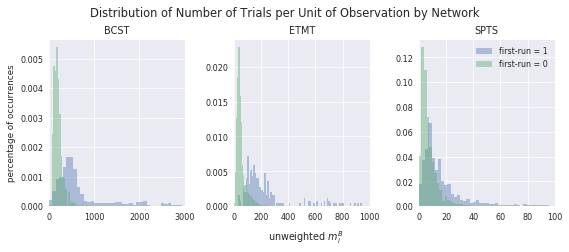
\includegraphics[scale=0.7]{kappa_explanation}
    \end{center}
    \caption{Distributions of the number of trials per each unit of observation factored
      by the covariate first-run.
      These distributions have much longer tails but have been truncated to illustrate the
      differences between each covariate factor's distribution. Note that the first-run units have a much wider distribution with
      a larger mean.
    }\label{fig:kappa:explanation}
  \end{figure}

\end{section}

\begin{section}{Inference}
  In order to compute the posterior density of our model, we perform the
  inference using the probabilistic programming language \texttt{pymc3} available through the programming language Python.
  This language
  allows us to specify the model $\mathcal{M}$ along with the observed data
  and also allows for the computation of the numerical approximation to the posterior density.

  \begin{subsection}{Computation}
    The computations of the approximation are performed through a Markov Chain Monte Carlo (MCMC) sampling algorithm.
    The algorithm itself is a variant of the Hamiltonian Monte Carlo (HMC) algorithm
    called the No U-Turn Sampler (NUTS). The description of the NUTS and HMC algorithms is beyond the scope of this
    paper, but the main idea is that the sampler borrows physical principles
    from Hamiltonian mechanics in combination with Monte Carlo simulation in order to compute the posterior density.
    The algorithm uses the Markov property to chooses the next point in the parameter space conditional
    only on the previous point \cite{pymc3}.

    An advantage of NUTS over regular HMC is that
    that the NUTS sampler has ``several self-tuning strategies
    for adaptively setting the tuneable parameters of Hamiltonian Monte Carlo.''
    This translates into the modeler only needing to specify the model and inferences are performed
    without much effort on the part of the modeler.

    The primary parameter available to the modeler to control the adaptation
    routines of the NUTS sampler is the \texttt{target\_accept} parameter. The value
    of this parameter determines the acceptance rate of the NUTS algorithm which is how often
    the sampler will accept target distributions during sampling. Higher values of this
    parameter correspond to smaller step sizes and allow the sampler to better explore
    the parameter space of the posterior density.

    The other parameters that are set include the number of ``tuned'' samples, the number of drawn samples,
    and the number of sampled Markov chains. The tuned samples are the simulations
    that are discarded and serve only to move the sampler away from the starting values
    of the Markov chain. Sampling from more than one Markov chain allows for convergence checks of the simulation
    as will be discussed
    in the next section. Once the sampler has been tuned, the algorithm draws the specified number of samples
    for each chain declared. After drawing the number of specified samples, the drawn parameters from the separate
    Markov chains are joined together to form the sampled posterior density.

    Throughout this paper, we set the above parameters as follows:
    \begin{itemize}
      \item \texttt{target\_accept}: 0.95
      \item tuned samples: 3000
      \item drawn samples: 500
      \item number of chains: 4
    \end{itemize}

  \end{subsection}

  \begin{subsection}{Convergence}
    Once we have performed the inference, we
    are interested in whether or not the simulation has approximately converged to
    the posterior density. Using samples from a simulation that has not converged
    carries the danger of biased inference which can lead to incorrect conclusions
    about the model.

    The main diagnostic check to determine if the sampler has approximately converged
    is the \emph{Gelman-Rubin} statistic, denoted by $\hat{R}$. This is a measure of
    the between-sequence and within-sequence variance across the Markov chains and is used to determine
    if stationarity and mixing has been achieved.

    Formally, for a model parameter $\psi$, suppose we have $N$ simulations
    and let $\{\phi_{ij}\}_{i=1}^{N}$ for $j=1\dots M$ simulated chains.
    The between-sequence and within-sequence variance is computed as
    \begin{align*}
      B = \frac{N}{M-1}\sum_{j=1}^M \left(\frac{1}{N}\sum_{i=1}^N\psi_{ij} - \frac{1}{MN}\sum_{j=1}^M \sum_{i=1}^N\psi_{ij}\right)^2 \\
      W = \frac{1}{M(N-1)}\sum_{j=1}^M\sum_{i=1}^N\left(\psi_{ij} - \frac{1}{N}\sum_{i=1}^N\psi_{ij}\right)^2
    \end{align*}
    respectively \cite{bda3}.
    Note that, $\text{Var}(\psi | y)$, the marginal posterior variance of the estimand $\psi$,
    can be estimated by a weighted average of $W$ and $B$, i.e.\
    \begin{align*}
      \hat{\text{Var}}^+(\psi | y) = \frac{N -1}{N} W + \frac{1}{N} B.
    \end{align*}
    which overestimate the marginal posterior variance, but is unbiased under stationarity
    or in the limit $N \to \infty$. However, the within variance $W$ should underestimate
    the marginal posterior variance since ``the individual sequences have not had time to range over
    all of the target distribution''. Thus, in the limit as $N \to \infty$,
    \begin{align}\label{form:rhat}
      \hat{R} = \sqrt{\frac{\hat{\text{Var}}^+(\psi | y)}{W}} \to 1,
    \end{align}
    and we can check for approximate convergence by determining if $\hat{R}$ is close to 1 \cite{bda3}.

    Another diagnostic check is the number of effective samples produced by the simulation, denoted
    by $n_{\text{eff}}$. Since the simulation draws within each sequence will have autocorrelation,
    the number of posterior samples is less than the simulation draws. Asymptotically, the effective
    sample size is
    \begin{align}\label{form:neff}
      n_{\text{eff}} = \frac{MN}{1 + 2 \sum_{t=1}^\infty \rho_t}
    \end{align}
    where $\rho_t$ is the autocorrelation of the simulation sequence at lag $t$ \cite{bda3}.
    The interested reader can consult Gelman et al.\
    for a technical discussion of how to calculate, $\hat{n_{\text{eff}}}$, an estimate of $n_{\text{eff}}$ for finite sequences.
    The recommendation from BDA3 is that $\hat{n_{\text{eff}}} > 10 M$, i.e.\ there are at least 10 independent
    draws for each sequence.

    For each network model, we have that $0.99 \leq \hat{R} \leq 1.01$ and $\hat{n_{\text{eff}}} > 400$
    for all model parameters. Thus, we conclude that the chains have mixed, are stationary,
    and that we have enough parameter samples to use to perform inference.
  \end{subsection}

\end{section}

\begin{section}{Validation}
  ``If the model fits, then replicated data under the model should look similar
  to observed data.'' \cite{bda3}
  Generating data using the posterior density of a model and then
  checking some aspect of the generated data set is similar to the analogous aspect
  of the observed data is called a posterior predictive check.

  Let $y$ be the observed data, $\theta$ be the vector of parameters, and $X$ be the model covariates.
  For model $\mathcal{M}$, we have that $\theta = (\pi, \omega, \kappa)$. Define $y^{\text{rep}}$
  to be the replicated data that could have generated given the vector of parameters $\theta$
  obtained through inference, i.e.\
  \begin{align}\label{form:yrep}
    p(y^{\text{rep}} | y) = \int p(y^{\text{rep}}|\theta)p(\theta | y) d\theta.
  \end{align}
  Note that since we use the posterior density obtained through inference to generate the replicated data sets,
  the replicated values are necessarily dependent on the observed data just as the posterior density is.

  The main purpose of posterior predictive checks is to measure the discrepancies between the
  data and the model and to determine if the discrepancies could have occurred by chance under the assumptions
  of the model \cite{bda3, kruschke}.

  \begin{subsection}{Replicated versus Actual Data Distributions}
    The first posterior predictive check we will perform is to assess whether the
    distribution of replicated data sets is similar to the distribution of observed data.
    We choose to graphically display these distributions for the assessment of the parameters
    $m_A^\text{rep}$ vs $m^A$, the observed data, and $c^{\text{rep}} = \pi$ vs $c$, the probability of a success for a given trial.
    Note that for each model we draw 500 simulated values from posterior predictive distribution.

    \begin{figure}[!h]
      \begin{subfigure}[b]{.75\textwidth}
        \centering
        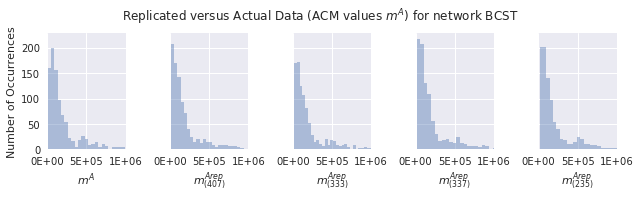
\includegraphics[scale=0.625]{BCST_m_rep}
      \end{subfigure}
      \begin{subfigure}[b]{.75\textwidth}
        \centering
        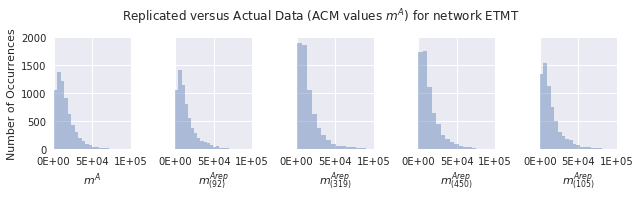
\includegraphics[scale=0.625]{ETMT_m_rep}
      \end{subfigure}
      \begin{subfigure}[b]{.75\textwidth}
        \centering
        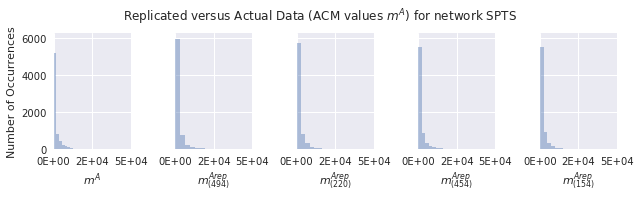
\includegraphics[scale=0.625]{SPTS_m_rep}
      \end{subfigure}
      \caption{Actual $m^A$ data (left) compared to replicated data sets $m^{A\text{rep}}$ (right four). Note that
        some parts of each distribution may be slightly truncated in order to display the critical features of the distribution.
        The replicated data sets largely mimic the actual data set.}
      \label{fig:m_rep}
    \end{figure}

    As can be seen from Figure \ref{fig:m_rep}, the replications $m_A^\text{rep}$ that have been drawn
    from the posterior density reasonably mimic the observed data. Thus, we see that in
    this aspect, the model is a good fit for the observed data.

    \begin{figure}[!h]
      \begin{subfigure}[b]{.75\textwidth}
        \centering
        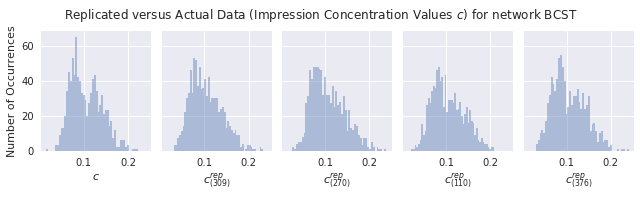
\includegraphics[scale=0.625]{BCST_c_rep}
      \end{subfigure}
      \begin{subfigure}[b]{.75\textwidth}
        \centering
        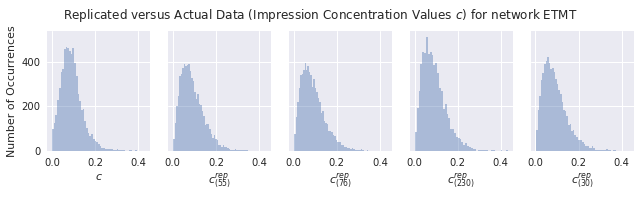
\includegraphics[scale=0.625]{ETMT_c_rep}
      \end{subfigure}
      \begin{subfigure}[b]{.75\textwidth}
        \centering
        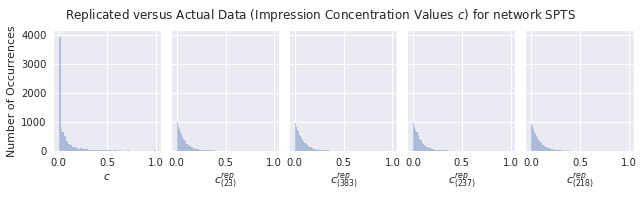
\includegraphics[scale=0.625]{SPTS_c_rep}
      \end{subfigure}
      \caption{Actual $c$ data (left) compared to the replicated data $c^{\text{rep}}$ (right four). The replicated
        data sets largely mimic the actual data set with the exception of the replicated data sets of network SPTS.}
      \label{fig:c_rep}
    \end{figure}

    Similarly, we see from Figure \ref{fig:c_rep} that the replications $c^{\text{rep}}$
    reasonably mimic the observed data with one notable exception; on the SPTS network,
    the replicated parameters $c^\text{rep}$ do not capture the mode of 0 in the observed data set.
    This is one aspect of the data that we do not wish to capture as we expect the probability
    of success to be positive, if only very small. The reasoning behind this is
    that the mode of 0 is present only due to the right censoring of the data, an artifact
    of the small number of trials present per unit of observation on the network. Thus, we accept this
    particular misfit of the model to the observed data and from the graphical replications
    declare that the model fits reasonably well.
  \end{subsection}

  \begin{subsection}{Test Statistics}\label{sec:test}
    We can also more concretely quantify model discrepancies by defining a test quantity $T(y, \theta)$
    and then measuring the discrepancy between the observed data and the replicated data.

    Formally, we can compute a posterior predictive $p$-value defined as
    \begin{align}\label{form:bayesp}
      p_B = \text{Pr}\left( T(y^{\text{rep}}, \theta) \geq T(y, \theta)  | y \right).
    \end{align}
    Values that exist in the extremes of 0 and 1 indicate poor model fit in regard to the particular
    aspect of the model that the test quantity aims to capture.
    As we have simulated values of the posterior density, the estimated $p$-value is
    just the proportion of the simulations such that the test quantity is greater than or equal
    to the test quantity as measured in the observed data, i.e.\
    \begin{align*}
      \hat{p_B} = \frac{1}{S}\sum_{i=1}^S [T(y_{(i)}^{\text{rep}}, \theta_{(i)}) \geq T(y, \theta_{(i)})]
    \end{align*}
    for $S$ simulations.

    We define the following test quantities to use in evaluating the fit of model $\mathcal{M}$:
    \begin{itemize}
      \item $T_1(y, \theta):= \min(y)$,
      \item $T_2(y, \theta):= \overline{y} = \frac{1}{N}\sum_{i=1}^N y_i$,
      \item $T_3(y, \theta):= \max(y)$,
      \item $T_4(y, \theta):= \text{std}(y) = \sqrt {\frac {\sum _{i=1}^{N}(y_{i}- \overline {y})^{2}}{N-1}}$,
      \item $T_5(y, \theta) := \overline{\pi} = \frac{1}{N}\sum_{i=1}^N \pi_i$.
    \end{itemize}

    In Table \ref{tab:bayesp} we summarize the results of these test quantities
    when compared to the observed data. As can be seen from the table, for some
    test quantities, the estimated $p$-value lie in the extremes. This suggests that the model
    does not fit those aspects of the data. For instance, on the ETMT network, the mean value of
    the replicated data are all greater than the mean of the observed data.

    \begin{sidewaystable}[!htbp]
      \centering
      \begin{tabular}{lrcccccccc}
        & \multicolumn{3}{c}{BCST network} & \multicolumn{3}{c}{ETMT network} & \multicolumn{3}{c}{SPTS network} \\
        Test quantity & $T(y, \theta)$ & \pbox{2cm}{95\% int. for $T(y^{\text{rep}}, \theta)$} & $p_B$ & $T(y, \theta)$ & \pbox{2cm}{95\% int. for $T(y^{\text{rep}}, \theta)$} & $p_B$  & $T(y)$ & \pbox{2cm}{95\% int. for $T(y^{\text{rep}}, \theta)$} & $p_B$ \\
        \hline
        $T_1(y, \theta)$ (min) & 3701 & [6245, 14270] & 0.99 & 0 & [9, 182] & 1.0 & 0 & [0, 0] & 1.0 \\
        $T_2(y, \theta)$ (mean) & 227457.84 & [2266852.49, 236367.09] & 0.95 & 16357.80 & [16705.39, 1748.11] & 1.0 & 3972.45 & [3714.91, 4559.66] & 0.73 \\
        $T_3(y, \theta)$ (max) & 4311038 & [3443885, 4989241] & 0.34 & 452762 & [307901, 760822] & 0.78 & 526816 & [607186, 2239365] & 0.99 \\
        $T_4(y, \theta)$ (std) & 334052.86 & [325128.37, 364859.10] & 0.90 & 17686.89 & [20021.24, 23205.09] & 1.0 & 22300.18 & [20012.59, 39808.44] & 0.88\\
        $T_5(y, \theta)$ (mean $\pi$)& 0.105 & [0.104, 0.107] & 0.60 & 0.0903 & [0.089, 0.092] & 0.43 & 0.056 & [0.065, 0.0689] & 1.0\\
      \end{tabular}
        \caption{Evaluation of test quantities across networks.}\label{tab:bayesp}
    \end{sidewaystable}
  \end{subsection}

    Note that there are pathological examples where the estimated $p$-values are 1,
    but do not adequately measure the discrepancy between
    the replicated data, e.g.\
    for the test statistic $T_1$ on the SPTS network, the estimated $p$-value is 1, but the replicated
    data matches the observed data in regards to this test statistic. Thus, we ignore such cases in evaluating the model fit.

    From these measured test quantities, we see that the model for BCST best fits the data and that
    the model does not adequately describe some aspects of the data for the other two networks.
    For the $p$-values of the test quantities that do lie in the extremes, the magnitude
    of the test quantity discrepancy is small. Thus, these models could be expanded to better accommodate
    the observed data, but we elect to use these models as is, noting that the
    model does not adequately describe all aspects of the observed data.

  \begin{subsection}{Regression Fit}
    The last check that we will perform is the analysis of the regression fit to the
    model. To evaluate this fit, we will analyze the standardized residuals of the model.

    For a model with unknown parameters $\theta$ and predictors $x_i$, the \emph{predicted}
    value is $\text{E}(y_i | x_i, \theta)$ and the \emph{residual} is $r_i = y_i - \text{E}(y_i | x_i, \theta)$.
    The $\emph{standardized residual}$ is given by $r_i / \text{std}(y)$ which allows us to
    ignore the magnitude of the data itself. Using the simulated posterior density,
    we can compute $\text{E}(y_i | x_i, \theta)$
    to be the mean of the replicated test, or hold-out, data itself.

    We can evaluate the standardized residuals by graphically comparing the replicated data from the hold-out set
    and their realized standardized residuals versus the observed data and their standardized residuals in the hold-out set.
    As we can see from Figure \ref{fig:res}, the standardized residuals have some misfits in the extremes of the data
    for the ETMT and SPTS network; as the replicated data becomes larger, so does the model's standardized residuals.

    \begin{figure}[!h]
      \begin{subfigure}[b]{.75\textwidth}
        \centering
        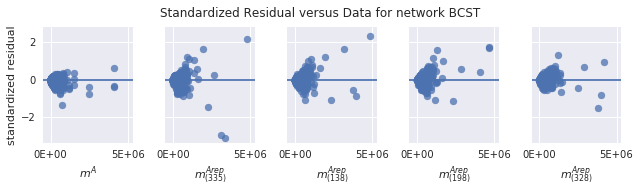
\includegraphics[scale=0.625]{BCST_res}
      \end{subfigure}
      \begin{subfigure}[b]{.75\textwidth}
        \centering
        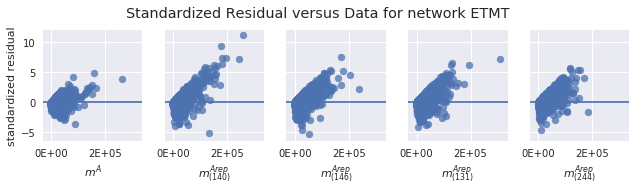
\includegraphics[scale=0.625]{ETMT_res}
      \end{subfigure}
      \begin{subfigure}[b]{.75\textwidth}
        \centering
        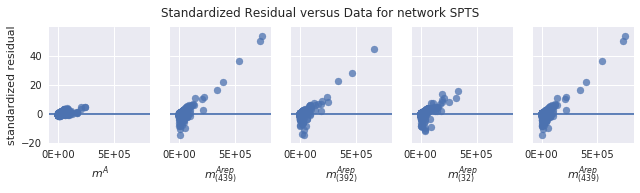
\includegraphics[scale=0.625]{SPTS_res}
      \end{subfigure}
      \caption{Actual standardized residuals data (left) compared to the standardized residuals of the replicated data (right four). For the ETMT and SPTS
        networks, the model's residuals become larger as the replicated becomes larger which is indicative of model misfit.}
      \label{fig:res}
    \end{figure}

    The misfit seen graphically can be quantified through the test quantity
    \begin{align*}
      T(y, \theta, x) = \frac{\overline{r}}{\text{std}(y)},
    \end{align*}
    which is the mean standardized residual of the data set. By proceeding as we did in Section \ref{sec:test},
    we can use \ref{form:bayesp} to calculate the estimated $p$-value of observing standardized residuals
    of the replicated test data set more extreme than in the observed data.

    \begin{figure}[!h]
      \begin{subfigure}[b]{.32\textwidth}
        \centering
        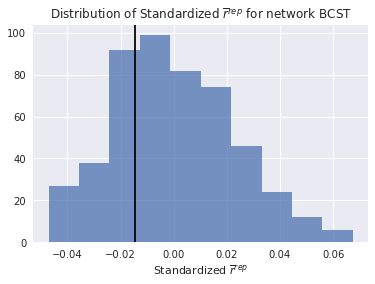
\includegraphics[scale=0.35]{BCST_res_test}
      \end{subfigure}
      \begin{subfigure}[b]{.32\textwidth}
        \centering
        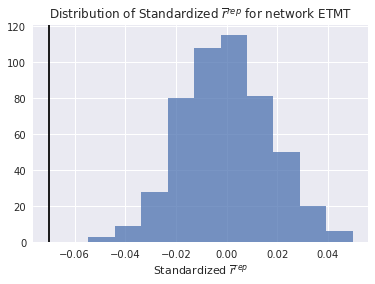
\includegraphics[scale=0.35]{ETMT_res_test}
      \end{subfigure}
      \begin{subfigure}[b]{.32\textwidth}
        \centering
        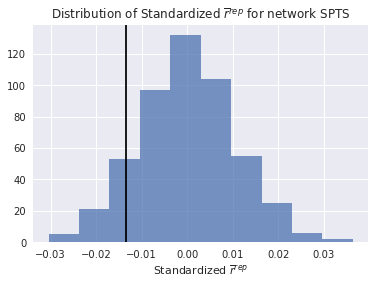
\includegraphics[scale=0.35]{SPTS_res_test}
      \end{subfigure}
      \caption{Graphical comparison of distribution of test quantities $T(y^{\text{rep}}, \theta, x)$ versus observed test quantity $T(y, \theta, x)$
        (black) in hold-out data set across networks.}
      \label{fig:restest}
    \end{figure}

    The graphical analysis of the above test quantities is shown in Figure \ref{fig:restest}. As we can see,
    for the BCST and SPTS networks, the standardized residuals of the replicated data sets do not
    differ in the extremes of the observed data set, while the standardized residuals do for the ETMT network.
    However, the magnitude of the discrepancy is small and we accept this deficiency of the model
    for the ETMT network. Note the results of the test quantities can be found in Table \ref{tab:bayesp_res}.

    \begin{table}[!htbp]
      \centering
      \begin{tabular}{lrcc}
        Network & $T(y, \theta, x)$ & \pbox{2cm}{95\% int. for $T(y^{\text{rep}}, \theta, x)$} & $p_B$ \\
        \hline
        BCST & -0.014 & [-0.043, 0.041] & 0.73 \\
        ETMT & -0.070 & [-0.030, 0.036] & 1.0 \\
        SPTS & -0.013 & [-0.022, 0.018] & 0.89 \\
      \end{tabular}
      \caption{Evaluation of test quantity $T(y, \theta, x)$ using the hold-out data set across networks.}
      \label{tab:bayesp_res}
    \end{table}

  \end{subsection}
\end{section}
\end{chapter}